\documentclass[oneside,a4paper,14pt]{extarticle}
\usepackage[T1,T2A]{fontenc}
\usepackage[
a4paper,
letterpaper,
top=2cm,
bottom=2cm,
left=2.5cm,
right=1.5cm
]{geometry}
\usepackage[utf8]{inputenc}
\usepackage[russian]{babel}
\usepackage{textcomp}
\usepackage{indentfirst}
\usepackage{listings}
\usepackage{xcolor}
\usepackage{enumitem}
\usepackage{graphicx}
\usepackage{mwe}
\usepackage{wrapfig}
\usepackage{caption}
\usepackage{amsmath}
\usepackage{amsfonts}
\usepackage{float}
\usepackage{amsthm}
\usepackage[all]{xy}
\usepackage[breaklinks]{hyperref}
\usepackage{titlesec}
\usepackage{adjustbox}
\usepackage{tikz}
\usetikzlibrary{positioning,arrows.meta,shapes.multipart}

\titleformat{\section}
{\normalsize\bfseries}
{\thesection} {1em}{}
\titleformat{\subsection}
{\normalsize\bfseries}
{\thesubsection} {1em}{}
\titleformat{\subsubsection}
{\normalsize\bfseries}
{\thesubsubsection} {1em}{}
\renewcommand\baselinestretch{1.33}
\normalsize
\setlength{\parindent}{1.25cm}

\lstset{
	language=SQL,
	basicstyle=\ttfamily\small,
	keywordstyle=\color{blue},
	commentstyle=\color{green!60!black},
	stringstyle=\color{red},
	numbers=left,
	numberstyle=\tiny\color{gray},
	frame=single,
	breaklines=true,
	showstringspaces=false,
	tabsize=4,
	inputencoding=utf8,
	extendedchars=true,
	literate={а}{{\selectfont\char224}}1 {б}{{\selectfont\char225}}1 {в}{{\selectfont\char226}}1 {г}{{\selectfont\char227}}1 {д}{{\selectfont\char228}}1 {е}{{\selectfont\char229}}1 {ё}{{\"e}}1 {ж}{{\selectfont\char230}}1 {з}{{\selectfont\char231}}1 {и}{{\selectfont\char232}}1 {й}{{\selectfont\char233}}1 {к}{{\selectfont\char234}}1 {л}{{\selectfont\char235}}1 {м}{{\selectfont\char236}}1 {н}{{\selectfont\char237}}1 {о}{{\selectfont\char238}}1 {п}{{\selectfont\char239}}1 {р}{{\selectfont\char240}}1 {с}{{\selectfont\char241}}1 {т}{{\selectfont\char242}}1 {у}{{\selectfont\char243}}1 {ф}{{\selectfont\char244}}1 {х}{{\selectfont\char245}}1 {ц}{{\selectfont\char246}}1 {ч}{{\selectfont\char247}}1 {ш}{{\selectfont\char248}}1 {щ}{{\selectfont\char249}}1 {ъ}{{\selectfont\char250}}1 {ы}{{\selectfont\char251}}1 {ь}{{\selectfont\char252}}1 {э}{{\selectfont\char253}}1 {ю}{{\selectfont\char254}}1 {я}{{\selectfont\char255}}1 {А}{{\selectfont\char192}}1 {Б}{{\selectfont\char193}}1 {В}{{\selectfont\char194}}1 {Г}{{\selectfont\char195}}1 {Д}{{\selectfont\char196}}1 {Е}{{\selectfont\char197}}1 {Ё}{{\"E}}1 {Ж}{{\selectfont\char198}}1 {З}{{\selectfont\char199}}1 {И}{{\selectfont\char200}}1 {Й}{{\selectfont\char201}}1 {К}{{\selectfont\char202}}1 {Л}{{\selectfont\char203}}1 {М}{{\selectfont\char204}}1 {Н}{{\selectfont\char205}}1 {О}{{\selectfont\char206}}1 {П}{{\selectfont\char207}}1 {Р}{{\selectfont\char208}}1 {С}{{\selectfont\char209}}1 {Т}{{\selectfont\char210}}1 {У}{{\selectfont\char211}}1 {Ф}{{\selectfont\char212}}1 {Х}{{\selectfont\char213}}1 {Ц}{{\selectfont\char214}}1 {Ч}{{\selectfont\char215}}1 {Ш}{{\selectfont\char216}}1 {Щ}{{\selectfont\char217}}1 {Ъ}{{\selectfont\char218}}1 {Ы}{{\selectfont\char219}}1 {Ь}{{\selectfont\char220}}1 {Э}{{\selectfont\char221}}1 {Ю}{{\selectfont\char222}}1 {Я}{{\selectfont\char223}}1 {«}{{\guillemotleft}}1 {»}{{\guillemotright}}1 {№}{{\textnumero}}1,
}

\begin{document}
	\sloppy
	\newpage\thispagestyle{empty}
	\begin{center}
		МИНИСТЕРСТВО НАУКИ И ВЫСШЕГО ОБРАЗОВАНИЯ\\
		РОССИЙСКОЙ ФЕДЕРАЦИИ\\
		ФЕДЕРАЛЬНОЕ ГОСУДАРСТВЕННОЕ БЮДЖЕТНОЕ\\
		ОБРАЗОВАТЕЛЬНОЕ УЧРЕЖДЕНИЕ ВЫСШЕГО ОБРАЗОВАНИЯ\\
		<<ВЯТСКИЙ ГОСУДАРСТВЕННЫЙ УНИВЕРСИТЕТ>>\\
		Институт математики и информационных систем\\
		Факультет автоматики и вычислительной техники\\
		Кафедра электронных вычислительных машин
	\end{center}
	\vspace{20mm}
	\begin{center}
		Отчёт по лабораторной работе №4\\
		по дисциплине\\
		<<Базы данных>>\\
	\end{center}
	\vspace{48mm}
	\noindent
	Выполнил студент гр. ИВТб-2303-06-00 \hfill \rule[-0,5mm]{30mm}{0.15mm}\,/Шубин В. Ю./
	\newline
	Проверил преподаватель кафедры ЭВМ \hfill \rule[-0,5mm]{30mm}{0.15mm}\,/Клюкин В. Л./
	\vfill
	\begin{center}
		Киров\\
		2026
	\end{center}
	\newpage
	\thispagestyle{empty}
	\section*{Цель работы:} Познакомиться с библиотекой Npgsql в C\# для связывания приложения с базой данных, изучить шаблоны проектирования, связанные с работой с БД, освоить на практике основы взаимодействия с БД под управлением PostgreSQL в приложении на C\# с графическим интерфейсом.
	
	\section*{Среда разработки:} PostgreSQL 18, pgAdmin 4, C\# (.NET Windows Forms, библиотека Npgsql), Windows 10.
	
	\newpage
	
	\section*{1. Архитектура приложения и диаграмма классов}
	
	Для работы с базой данных \texttt{lab\_db} (схема \texttt{lab\_schema}) выбрана таблица \texttt{game} («Видеоигры»), содержащая внешний ключ \texttt{developer\_id} на родительскую таблицу \texttt{developer} («Разработчики»).
	
	При проектировании приложения применён шаблон проектирования \textbf{Repository} (\textbf{Репозиторий / Data Access Object}) и \textbf{Factory Method} (\textbf{Фабричный метод}):
	\begin{itemize}
		\item \texttt{Developer} и \texttt{Game} --- классы сущностей предметной области (Domain Model), представляющие записи таблиц \texttt{developer} и \texttt{game};
		\item \texttt{DbConnectionFactory} --- фабрика подключений, создающая и открывающая соединения \texttt{NpgsqlConnection};
		\item \texttt{DeveloperRepository} --- репозиторий для чтения списка разработчиков из родительской таблицы \texttt{developer};
		\item \texttt{GameRepository} --- репозиторий для чтения, регистронезависимой фильтрации через SQL-запрос, проверки дубликатов, а также сохранения и удаления записей таблицы \texttt{game} с использованием функций PL/pgSQL;
		\item \texttt{Form1} --- класс главной экранной формы графического интерфейса.
	\end{itemize}
	
	Диаграмма разработанных классов, организующих взаимодействие с БД, представлена на рисунке~1.
	
	\begin{figure}[H]
		\centering
		\begin{adjustbox}{max width=\linewidth}
		\begin{tikzpicture}[
			classbox/.style={
				rectangle split,
				rectangle split parts=3,
				draw=black,
				thick,
				fill=white,
				font=\ttfamily\scriptsize,
				align=left,
				inner sep=6pt
			},
			rel/.style={-{Stealth[length=3mm, width=2.2mm]}, thick},
			dep/.style={-{Stealth[length=3mm, width=2.2mm]}, thick, dashed}
		]
			% Top: Form1
			\node[classbox, text width=9.2cm] (form) at (0, 0) {
				\textbf{\centerline{Form1}}
				\nodepart{second}
				- \_developerRepository : DeveloperRepository\\
				- \_gameRepository : GameRepository\\
				- \_currentGameId : long?
				\nodepart{third}
				+ LoadDevelopers() : void\\
				+ LoadGames(filter : string) : void\\
				+ ValidateInput(out year : int, out price : decimal) : bool\\
				+ ClearFields() : void\\
				- btnAdd\_Click(sender : object, e : EventArgs) : void\\
				- btnUpdate\_Click(sender : object, e : EventArgs) : void\\
				- btnDelete\_Click(sender : object, e : EventArgs) : void\\
				- btnFilter\_Click(sender : object, e : EventArgs) : void\\
				- txtNumeric\_KeyPress(sender : object, e : KeyPressEventArgs) : void
			};

			% Middle: Repositories
			\node[classbox, text width=7.5cm] (devRepo) at (-5.2, -5.8) {
				\textbf{\centerline{DeveloperRepository}}
				\nodepart{second}
				- \_connectionFactory : DbConnectionFactory
				\nodepart{third}
				+ DeveloperRepository(factory : DbConnectionFactory)\\
				+ GetAll() : List<Developer>
			};

			\node[classbox, text width=8.2cm] (gameRepo) at (5.0, -6.5) {
				\textbf{\centerline{GameRepository}}
				\nodepart{second}
				- \_connectionFactory : DbConnectionFactory
				\nodepart{third}
				+ GameRepository(factory : DbConnectionFactory)\\
				+ GetAll() : List<Game>\\
				+ FilterByTitle(titlePattern : string) : List<Game>\\
				+ ExistsByTitle(title : string, excludeId : long?) : bool\\
				+ Save(game : Game) : long\\
				+ Delete(id : long) : void
			};

			% Bottom row: Developer, DbConnectionFactory, Game
			\node[classbox, text width=5.2cm] (dev) at (-6.8, -12.2) {
				\textbf{\centerline{Developer}}
				\nodepart{second}
				+ Id : long\\
				+ Name : string
				\nodepart{third}
				+ Developer(id : long, name : string)\\
				+ ToString() : string
			};

			\node[classbox, text width=5.8cm] (factory) at (0.0, -12.2) {
				\textbf{\centerline{DbConnectionFactory}}
				\nodepart{second}
				- \_connectionString : string
				\nodepart{third}
				+ DbConnectionFactory(connStr : string)\\
				+ CreateConnection() : NpgsqlConnection
			};

			\node[classbox, text width=5.4cm] (game) at (6.8, -12.9) {
				\textbf{\centerline{Game}}
				\nodepart{second}
				+ Id : long?\\
				+ Title : string\\
				+ DeveloperId : long\\
				+ DeveloperName : string\\
				+ ReleaseYear : int\\
				+ Price : decimal\\
				+ IsReleased : bool
				\nodepart{third}
				+ Game(...)
			};

			% Arrows
			\draw[rel] (form.south) -- ++(0,-0.7) -| (devRepo.north);
			\draw[rel] (form.south) -- ++(0,-0.7) -| (gameRepo.north);

			\draw[dep] (devRepo.south) -- (dev.north);
			\draw[rel] (devRepo.south east) -- (factory.north west);

			\draw[rel] (gameRepo.south west) -- (factory.north east);
			\draw[dep] (gameRepo.south) -- (game.north);
		\end{tikzpicture}
		\end{adjustbox}
		\caption{Диаграмма разработанных классов, организующих взаимодействие с БД}
	\end{figure}
	
	\newpage
	
	\section*{2. Хранимые функции PL/pgSQL для работы с БД}
	
	Чтение данных, регистронезависимая фильтрация с использованием функции \texttt{UPPER}, сохранение (вставка и изменение) и удаление строк реализованы на стороне СУБД PostgreSQL с помощью функций на языке PL/pgSQL.
	
	\begin{lstlisting}[language=SQL]
-- 1. Получение списка всех разработчиков (родительская таблица)
CREATE OR REPLACE FUNCTION lab_schema.get_all_developers()
RETURNS TABLE(
    id BIGINT,
    name VARCHAR(100)
) AS $$
BEGIN
    RETURN QUERY
    SELECT d.id, d.name
    FROM lab_schema.developer d
    ORDER BY d.name;
END;
$$ LANGUAGE plpgsql;

-- 2. Получение списка всех игр с названиями разработчиков
CREATE OR REPLACE FUNCTION lab_schema.get_games_with_developers()
RETURNS TABLE(
    id BIGINT,
    title VARCHAR(150),
    developer_name VARCHAR(100),
    release_year INTEGER,
    price NUMERIC(10, 2),
    is_released BOOLEAN
) AS $$
BEGIN
    RETURN QUERY
    SELECT g.id, g.title, d.name, g.release_year, g.price, g.is_released
    FROM lab_schema.game g
    JOIN lab_schema.developer d ON g.developer_id = d.id
    ORDER BY g.id;
END;
$$ LANGUAGE plpgsql;

-- 3. Регистронезависимая фильтрация игр по названию (с использованием UPPER)
CREATE OR REPLACE FUNCTION lab_schema.filter_games_by_title(
    _title_pattern VARCHAR(150)
)
RETURNS TABLE(
    id BIGINT,
    title VARCHAR(150),
    developer_name VARCHAR(100),
    release_year INTEGER,
    price NUMERIC(10, 2),
    is_released BOOLEAN
) AS $$
BEGIN
    RETURN QUERY
    SELECT g.id, g.title, d.name, g.release_year, g.price, g.is_released
    FROM lab_schema.game g
    JOIN lab_schema.developer d ON g.developer_id = d.id
    WHERE UPPER(g.title) LIKE UPPER(_title_pattern)
    ORDER BY g.id;
END;
$$ LANGUAGE plpgsql;

-- 4. Сохранение (добавление или изменение) строки таблицы game
CREATE OR REPLACE FUNCTION lab_schema.save_game(
    _id BIGINT,
    _title VARCHAR(150),
    _developer_id BIGINT,
    _release_year INTEGER,
    _price NUMERIC(10, 2),
    _is_released BOOLEAN
)
RETURNS BIGINT AS $$
DECLARE
    used_id BIGINT;
BEGIN
    IF EXISTS (
        SELECT 1 FROM lab_schema.game
        WHERE UPPER(TRIM(title)) = UPPER(TRIM(_title))
          AND (_id IS NULL OR id <> _id)
    ) THEN
        RAISE EXCEPTION 'Игра с названием "%" уже существует в базе данных!', _title;
    END IF;

    IF _id IS NULL THEN
        INSERT INTO lab_schema.game (title, developer_id, release_year, price, is_released)
        VALUES (TRIM(_title), _developer_id, _release_year, _price, _is_released)
        RETURNING id INTO used_id;
    ELSE
        UPDATE lab_schema.game
        SET title = TRIM(_title),
            developer_id = _developer_id,
            release_year = _release_year,
            price = _price,
            is_released = _is_released
        WHERE id = _id;
        used_id := _id;
    END IF;

    RETURN used_id;
END;
$$ LANGUAGE plpgsql;

-- 5. Удаление строки таблицы game по id
CREATE OR REPLACE FUNCTION lab_schema.delete_game(
    _id BIGINT
)
RETURNS VOID AS $$
BEGIN
    DELETE FROM lab_schema.log_game WHERE game_id = _id;
    DELETE FROM lab_schema.game WHERE id = _id;
EXCEPTION
    WHEN foreign_key_violation THEN
        RAISE EXCEPTION 'Невозможно удалить игру, так как на неё есть ссылки из других таблиц.';
END;
$$ LANGUAGE plpgsql;
	\end{lstlisting}
	
	\newpage
	
	\section*{3. Исходный код классов приложения на C\#}
	
	Ниже приведён исходный код классов сущностей (\texttt{Developer.cs}, \texttt{Game.cs}), фабрики подключений (\texttt{DbConnectionFactory.cs}), а также репозиториев (\texttt{DeveloperRepository.cs}, \texttt{GameRepository.cs}) и главной экранной формы приложения (\texttt{Form1.cs}).
	
	\subsection*{Классы сущностей Developer и Game}
	\begin{lstlisting}[language={[Sharp]C}]
using System;

namespace VideoGamesApp
{
    // Класс сущности «Разработчик» (родительская таблица lab_schema.developer)
    public class Developer
    {
        public long Id { get; set; }
        public string Name { get; set; }

        public Developer() { }

        public Developer(long id, string name)
        {
            Id = id;
            Name = name;
        }

        public override string ToString()
        {
            return Name;
        }
    }

    // Класс сущности «Видеоигра» (дочерняя таблица lab_schema.game)
    public class Game
    {
        public long? Id { get; set; }
        public string Title { get; set; }
        public long DeveloperId { get; set; }
        public string DeveloperName { get; set; }
        public int ReleaseYear { get; set; }
        public decimal Price { get; set; }
        public bool IsReleased { get; set; }

        public Game() { }

        public Game(long? id, string title, long developerId, string developerName,
                    int releaseYear, decimal price, bool isReleased)
        {
            Id = id;
            Title = title;
            DeveloperId = developerId;
            DeveloperName = developerName;
            ReleaseYear = releaseYear;
            Price = price;
            IsReleased = isReleased;
        }
    }
}
	\end{lstlisting}
	
	\subsection*{Классы DbConnectionFactory и DeveloperRepository}
	\begin{lstlisting}[language={[Sharp]C}]
using System.Collections.Generic;
using Npgsql;

namespace VideoGamesApp
{
    // Фабрика подключений к базе данных PostgreSQL
    public class DbConnectionFactory
    {
        private readonly string _connectionString;

        public DbConnectionFactory(string connectionString)
        {
            _connectionString = connectionString;
        }

        public NpgsqlConnection CreateConnection()
        {
            NpgsqlConnection conn = new NpgsqlConnection(_connectionString);
            conn.Open();
            return conn;
        }
    }

    // Репозиторий для работы с родительской таблицей разработчиков
    public class DeveloperRepository
    {
        private readonly DbConnectionFactory _connectionFactory;

        public DeveloperRepository(DbConnectionFactory connectionFactory)
        {
            _connectionFactory = connectionFactory;
        }

        public List<Developer> GetAll()
        {
            List<Developer> developers = new List<Developer>();
            NpgsqlConnection conn = _connectionFactory.CreateConnection();
            try
            {
                NpgsqlCommand cmd = new NpgsqlCommand(
                    "SELECT * FROM lab_schema.get_all_developers()", conn);
                NpgsqlDataReader reader = cmd.ExecuteReader();
                while (reader.Read())
                {
                    long id = reader.GetInt64(0);
                    string name = reader.GetString(1);
                    developers.Add(new Developer(id, name));
                }
                reader.Close();
            }
            finally
            {
                conn.Close();
            }
            return developers;
        }
    }
}
	\end{lstlisting}
	
	\subsection*{Класс GameRepository}
	\begin{lstlisting}[language={[Sharp]C}]
using System;
using System.Collections.Generic;
using Npgsql;
using NpgsqlTypes;

namespace VideoGamesApp
{
    // Репозиторий для работы с таблицей видеоигр (lab_schema.game)
    public class GameRepository
    {
        private readonly DbConnectionFactory _connectionFactory;

        public GameRepository(DbConnectionFactory connectionFactory)
        {
            _connectionFactory = connectionFactory;
        }

        // Получение всех записей таблицы game с названиями разработчиков
        public List<Game> GetAll()
        {
            List<Game> games = new List<Game>();
            NpgsqlConnection conn = _connectionFactory.CreateConnection();
            try
            {
                NpgsqlCommand cmd = new NpgsqlCommand(
                    "SELECT * FROM lab_schema.get_games_with_developers()", conn);
                NpgsqlDataReader reader = cmd.ExecuteReader();
                while (reader.Read())
                {
                    games.Add(new Game(
                        reader.GetInt64(0),
                        reader.GetString(1),
                        0,
                        reader.GetString(2),
                        reader.GetInt32(3),
                        reader.GetDecimal(4),
                        reader.GetBoolean(5)
                    ));
                }
                reader.Close();
            }
            finally
            {
                conn.Close();
            }
            return games;
        }

        // Регистронезависимая фильтрация по названию через запрос к БД
        public List<Game> FilterByTitle(string titlePattern)
        {
            List<Game> games = new List<Game>();
            NpgsqlConnection conn = _connectionFactory.CreateConnection();
            try
            {
                NpgsqlCommand cmd = new NpgsqlCommand(
                    "SELECT * FROM lab_schema.filter_games_by_title(@pattern)", conn);
                NpgsqlParameter paramPattern = new NpgsqlParameter("@pattern", NpgsqlDbType.Varchar);
                paramPattern.Value = "%" + titlePattern + "%";
                cmd.Parameters.Add(paramPattern);

                NpgsqlDataReader reader = cmd.ExecuteReader();
                while (reader.Read())
                {
                    games.Add(new Game(
                        reader.GetInt64(0),
                        reader.GetString(1),
                        0,
                        reader.GetString(2),
                        reader.GetInt32(3),
                        reader.GetDecimal(4),
                        reader.GetBoolean(5)
                    ));
                }
                reader.Close();
            }
            finally
            {
                conn.Close();
            }
            return games;
        }

        // Проверка наличия дубликата в БД (без учёта регистра)
        public bool ExistsByTitle(string title, long? excludeId = null)
        {
            NpgsqlConnection conn = _connectionFactory.CreateConnection();
            try
            {
                string sql = @"SELECT EXISTS (
                    SELECT 1 FROM lab_schema.game
                    WHERE UPPER(TRIM(title)) = UPPER(TRIM(@title))
                      AND (@exclude_id IS NULL OR id <> @exclude_id)
                )";
                NpgsqlCommand cmd = new NpgsqlCommand(sql, conn);

                NpgsqlParameter paramTitle = new NpgsqlParameter("@title", NpgsqlDbType.Varchar);
                paramTitle.Value = title.Trim();
                cmd.Parameters.Add(paramTitle);

                NpgsqlParameter paramExcludeId = new NpgsqlParameter("@exclude_id", NpgsqlDbType.Bigint);
                paramExcludeId.Value = excludeId.HasValue ? (object)excludeId.Value : DBNull.Value;
                cmd.Parameters.Add(paramExcludeId);

                object result = cmd.ExecuteScalar();
                return result != null && Convert.ToBoolean(result);
            }
            finally
            {
                conn.Close();
            }
        }

        // Сохранение строки с помощью функции PL/pgSQL save_game
        public long Save(Game game)
        {
            NpgsqlConnection conn = _connectionFactory.CreateConnection();
            try
            {
                NpgsqlCommand cmd = new NpgsqlCommand(
                    "SELECT lab_schema.save_game(@id, @title, @dev_id, @year, @price, @released)", conn);

                NpgsqlParameter pId = new NpgsqlParameter("@id", NpgsqlDbType.Bigint);
                pId.Value = game.Id.HasValue ? (object)game.Id.Value : DBNull.Value;
                cmd.Parameters.Add(pId);

                NpgsqlParameter pTitle = new NpgsqlParameter("@title", NpgsqlDbType.Varchar);
                pTitle.Value = game.Title.Trim();
                cmd.Parameters.Add(pTitle);

                NpgsqlParameter pDevId = new NpgsqlParameter("@dev_id", NpgsqlDbType.Bigint);
                pDevId.Value = game.DeveloperId;
                cmd.Parameters.Add(pDevId);

                NpgsqlParameter pYear = new NpgsqlParameter("@year", NpgsqlDbType.Integer);
                pYear.Value = game.ReleaseYear;
                cmd.Parameters.Add(pYear);

                NpgsqlParameter pPrice = new NpgsqlParameter("@price", NpgsqlDbType.Numeric);
                pPrice.Value = game.Price;
                cmd.Parameters.Add(pPrice);

                NpgsqlParameter pReleased = new NpgsqlParameter("@released", NpgsqlDbType.Boolean);
                pReleased.Value = game.IsReleased;
                cmd.Parameters.Add(pReleased);

                object result = cmd.ExecuteScalar();
                return Convert.ToInt64(result);
            }
            finally
            {
                conn.Close();
            }
        }

        // Удаление строки с помощью функции PL/pgSQL delete_game
        public void Delete(long id)
        {
            NpgsqlConnection conn = _connectionFactory.CreateConnection();
            try
            {
                NpgsqlCommand cmd = new NpgsqlCommand("SELECT lab_schema.delete_game(@id)", conn);
                NpgsqlParameter pId = new NpgsqlParameter("@id", NpgsqlDbType.Bigint);
                pId.Value = id;
                cmd.Parameters.Add(pId);

                cmd.ExecuteNonQuery();
            }
            finally
            {
                conn.Close();
            }
        }
    }
}
	\end{lstlisting}
	
	\subsection*{Класс экранной формы Form1}
	\begin{lstlisting}[language={[Sharp]C}]
using System;
using System.Collections.Generic;
using System.Globalization;
using System.Windows.Forms;

namespace VideoGamesApp
{
    public partial class Form1 : Form
    {
        private const string ConnectionString =
            "Server=127.0.0.1;Port=5432;User Id=lab_test;Password=lab_test;Database=lab_db";

        private readonly DeveloperRepository _developerRepository;
        private readonly GameRepository _gameRepository;
        private long? _currentGameId = null;

        public Form1()
        {
            InitializeComponent();

            DbConnectionFactory connectionFactory = new DbConnectionFactory(ConnectionString);
            _developerRepository = new DeveloperRepository(connectionFactory);
            _gameRepository = new GameRepository(connectionFactory);

            LoadDevelopers();
            LoadGames();
        }

        public void LoadDevelopers()
        {
            try
            {
                List<Developer> developers = _developerRepository.GetAll();
                cmbDeveloper.Items.Clear();
                foreach (Developer dev in developers)
                {
                    cmbDeveloper.Items.Add(dev);
                }
            }
            catch (Exception ex)
            {
                MessageBox.Show($"Ошибка загрузки разработчиков: {ex.Message}",
                    "Ошибка", MessageBoxButtons.OK, MessageBoxIcon.Error);
            }
        }

        public void LoadGames(string filter = null)
        {
            try
            {
                List<Game> games = string.IsNullOrEmpty(filter)
                    ? _gameRepository.GetAll()
                    : _gameRepository.FilterByTitle(filter);

                dgvGames.Rows.Clear();
                foreach (Game game in games)
                {
                    dgvGames.Rows.Add(
                        game.Id,
                        game.Title,
                        game.DeveloperName,
                        game.ReleaseYear,
                        game.Price.ToString("0.00"),
                        game.IsReleased ? "Да" : "Нет"
                    );
                }
            }
            catch (Exception ex)
            {
                MessageBox.Show($"Ошибка загрузки игр: {ex.Message}",
                    "Ошибка", MessageBoxButtons.OK, MessageBoxIcon.Error);
            }
        }

        // Запрет ввода знака минус (отрицательных значений)
        private void txtNumeric_KeyPress(object sender, KeyPressEventArgs e)
        {
            if (e.KeyChar == '-')
            {
                e.Handled = true;
                MessageBox.Show("Ввод отрицательных значений запрещён!",
                    "Ограничение ввода", MessageBoxButtons.OK, MessageBoxIcon.Warning);
            }
        }

        private void btnAdd_Click(object sender, EventArgs e)
        {
            if (!ValidateInput(out int year, out decimal price))
                return;

            string title = txtTitle.Text.Trim();
            Developer selectedDev = (Developer)cmbDeveloper.SelectedItem;

            try
            {
                if (_gameRepository.ExistsByTitle(title, null))
                {
                    MessageBox.Show(
                        $"Игра с названием «{title}» уже существует в базе данных! Запись данных в таблицу не выполнена.",
                        "Дублирование данных", MessageBoxButtons.OK, MessageBoxIcon.Warning);
                    return;
                }

                Game newGame = new Game(null, title, selectedDev.Id, selectedDev.Name, year, price, chkReleased.Checked);
                _gameRepository.Save(newGame);

                MessageBox.Show("Игра успешно добавлена!",
                    "Успех", MessageBoxButtons.OK, MessageBoxIcon.Information);
                ClearFields();
                LoadGames();
            }
            catch (Exception ex)
            {
                MessageBox.Show($"Ошибка добавления: {ex.Message}",
                    "Ошибка", MessageBoxButtons.OK, MessageBoxIcon.Error);
            }
        }

        private void btnUpdate_Click(object sender, EventArgs e)
        {
            if (_currentGameId == null)
            {
                MessageBox.Show("Выберите игру в таблице для изменения!",
                    "Предупреждение", MessageBoxButtons.OK, MessageBoxIcon.Warning);
                return;
            }

            if (!ValidateInput(out int year, out decimal price))
                return;

            string title = txtTitle.Text.Trim();
            Developer selectedDev = (Developer)cmbDeveloper.SelectedItem;

            try
            {
                if (_gameRepository.ExistsByTitle(title, _currentGameId))
                {
                    MessageBox.Show(
                        $"Другая игра с названием «{title}» уже существует в базе данных! Изменение не сохранено.",
                        "Дублирование данных", MessageBoxButtons.OK, MessageBoxIcon.Warning);
                    return;
                }

                Game updatedGame = new Game(_currentGameId, title, selectedDev.Id, selectedDev.Name, year, price, chkReleased.Checked);
                _gameRepository.Save(updatedGame);

                MessageBox.Show("Данные игры успешно изменены!",
                    "Успех", MessageBoxButtons.OK, MessageBoxIcon.Information);
                ClearFields();
                LoadGames();
            }
            catch (Exception ex)
            {
                MessageBox.Show($"Ошибка изменения: {ex.Message}",
                    "Ошибка", MessageBoxButtons.OK, MessageBoxIcon.Error);
            }
        }

        private void btnDelete_Click(object sender, EventArgs e)
        {
            if (_currentGameId == null)
            {
                MessageBox.Show("Выберите игру в таблице для удаления!",
                    "Предупреждение", MessageBoxButtons.OK, MessageBoxIcon.Warning);
                return;
            }

            DialogResult result = MessageBox.Show(
                "Вы действительно уверены, что хотите удалить выбранную запись?",
                "Подтверждение удаления", MessageBoxButtons.YesNo, MessageBoxIcon.Question);

            if (result == DialogResult.Yes)
            {
                try
                {
                    _gameRepository.Delete(_currentGameId.Value);
                    MessageBox.Show("Запись успешно удалена!",
                        "Успех", MessageBoxButtons.OK, MessageBoxIcon.Information);
                    ClearFields();
                    LoadGames();
                }
                catch (Exception ex)
                {
                    MessageBox.Show($"Ошибка удаления: {ex.Message}",
                        "Ошибка", MessageBoxButtons.OK, MessageBoxIcon.Error);
                }
            }
        }

        private void btnClear_Click(object sender, EventArgs e)
        {
            ClearFields();
        }

        private void btnFilter_Click(object sender, EventArgs e)
        {
            string filter = txtFilter.Text.Trim();
            LoadGames(string.IsNullOrEmpty(filter) ? null : filter);
        }

        private void btnResetFilter_Click(object sender, EventArgs e)
        {
            txtFilter.Text = "";
            LoadGames();
        }

        private void dgvGames_CellClick(object sender, DataGridViewCellEventArgs e)
        {
            if (e.RowIndex >= 0)
            {
                SelectRow(e.RowIndex);
            }
        }

        public void SelectRow(int rowIndex)
        {
            if (rowIndex >= 0 && rowIndex < dgvGames.Rows.Count)
            {
                dgvGames.ClearSelection();
                dgvGames.Rows[rowIndex].Selected = true;

                _currentGameId = Convert.ToInt64(dgvGames.Rows[rowIndex].Cells[0].Value);
                txtTitle.Text = dgvGames.Rows[rowIndex].Cells[1].Value.ToString();

                string devName = dgvGames.Rows[rowIndex].Cells[2].Value.ToString();
                foreach (Developer item in cmbDeveloper.Items)
                {
                    if (item.Name == devName)
                    {
                        cmbDeveloper.SelectedItem = item;
                        break;
                    }
                }

                txtYear.Text = dgvGames.Rows[rowIndex].Cells[3].Value.ToString();
                txtPrice.Text = dgvGames.Rows[rowIndex].Cells[4].Value.ToString();
                chkReleased.Checked = dgvGames.Rows[rowIndex].Cells[5].Value.ToString() == "Да";
            }
        }

        public bool ValidateInput(out int year, out decimal price)
        {
            year = 0;
            price = 0m;

            if (string.IsNullOrWhiteSpace(txtTitle.Text))
            {
                MessageBox.Show("Введите название игры!",
                    "Ошибка ввода", MessageBoxButtons.OK, MessageBoxIcon.Warning);
                return false;
            }

            if (cmbDeveloper.SelectedItem == null)
            {
                MessageBox.Show("Выберите разработчика из списка!",
                    "Ошибка ввода", MessageBoxButtons.OK, MessageBoxIcon.Warning);
                return false;
            }

            if (!int.TryParse(txtYear.Text.Trim(), out year))
            {
                MessageBox.Show("Год выпуска должен быть целым числом!",
                    "Ошибка ввода", MessageBoxButtons.OK, MessageBoxIcon.Warning);
                return false;
            }

            if (year < 0)
            {
                MessageBox.Show("Год выпуска не может быть отрицательным значением!",
                    "Ошибка ввода", MessageBoxButtons.OK, MessageBoxIcon.Warning);
                return false;
            }

            if (year < 1970 || year > 2030)
            {
                MessageBox.Show("Год выпуска должен находиться в диапазоне от 1970 до 2030!",
                    "Ошибка ввода", MessageBoxButtons.OK, MessageBoxIcon.Warning);
                return false;
            }

            string rawPrice = txtPrice.Text.Trim().Replace(',', '.');
            if (!decimal.TryParse(rawPrice, NumberStyles.Number, CultureInfo.InvariantCulture, out price))
            {
                MessageBox.Show("Введите корректное числовое значение цены!",
                    "Ошибка ввода", MessageBoxButtons.OK, MessageBoxIcon.Warning);
                return false;
            }

            if (price < 0)
            {
                MessageBox.Show("Цена не может быть отрицательной!",
                    "Ошибка ввода", MessageBoxButtons.OK, MessageBoxIcon.Warning);
                return false;
            }

            return true;
        }

        public void ClearFields()
        {
            _currentGameId = null;
            txtTitle.Text = "";
            cmbDeveloper.SelectedIndex = -1;
            txtYear.Text = "";
            txtPrice.Text = "";
            chkReleased.Checked = false;
        }
    }
}
	\end{lstlisting}
	
	\newpage
	
	\section*{4. Экранные формы работы приложения}
	
	Главное окно приложения после запуска и загрузки записей таблицы \texttt{game} представлено на рисунке~2. Все названия колонок, кнопок и подписей элементов управления выполнены на русском языке, а внешний ключ (\texttt{Разработчик}) отображается и выбирается по названию из родительской таблицы \texttt{developer}.
	
	\begin{figure}[H]
		\centering
		\adjustbox{max width=0.92\linewidth}{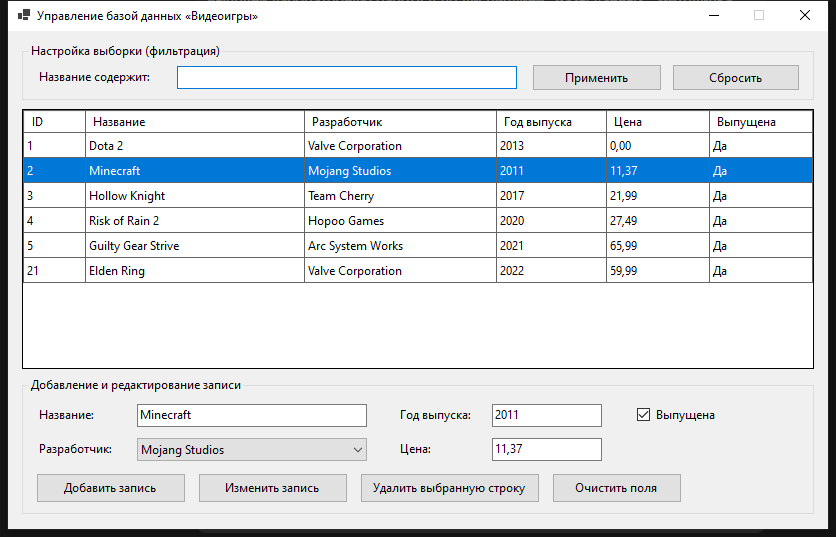
\includegraphics{s1.png}}
		\caption{Главная экранная форма приложения с загруженными данными}
	\end{figure}
	
	Результат добавления новой записи в таблицу \texttt{game} с выбором разработчика из выпадающего списка \texttt{ComboBox} и вызовом функции \texttt{lab\_schema.save\_game} представлен на рисунке~3.
	
	\begin{figure}[H]
		\centering
		\adjustbox{max width=0.92\linewidth}{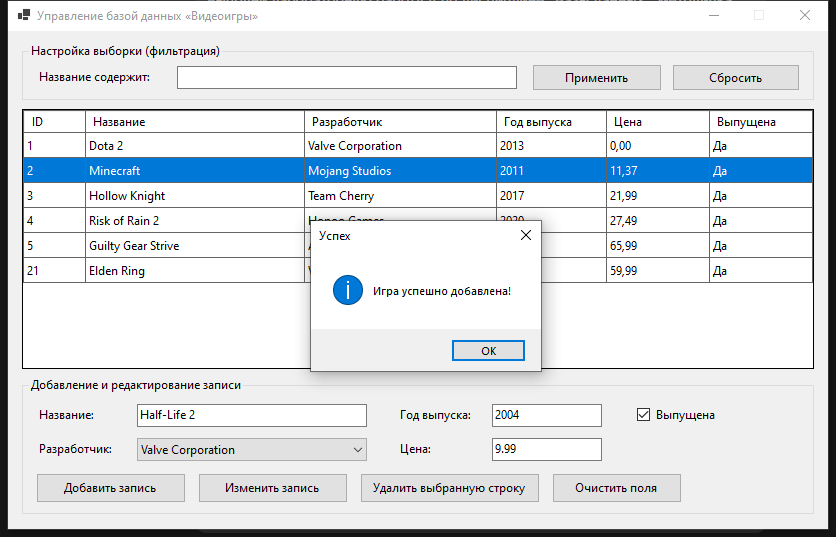
\includegraphics{s2.png}}
		\caption{Добавление новой записи в таблицу}
	\end{figure}
	
	При попытке повторного ввода уже имеющихся в таблице данных пользователю выводится предупреждающее сообщение без записи дубликата в таблицу (рисунок~4).
	
	\begin{figure}[H]
		\centering
		\adjustbox{max width=0.92\linewidth}{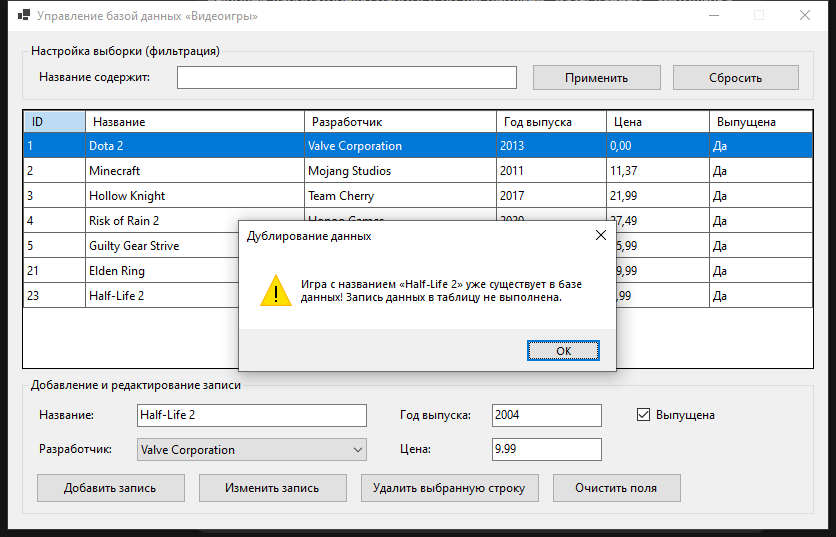
\includegraphics{s3.png}}
		\caption{Сообщение при попытке ввода уже имеющихся данных}
	\end{figure}
	
	Проверка запрета ввода отрицательных значений для числового поля «Цена» представлена на рисунке~5.
	
	\begin{figure}[H]
		\centering
		\adjustbox{max width=0.92\linewidth}{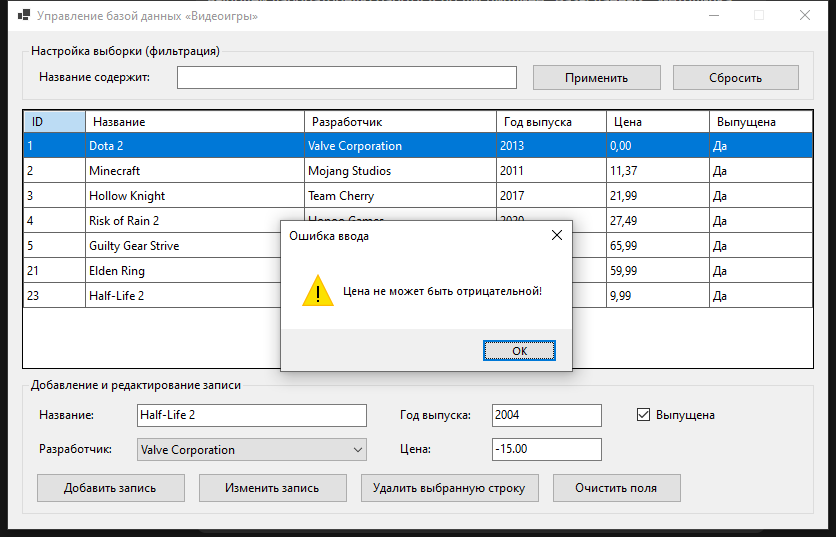
\includegraphics{s4.png}}
		\caption{Запрет ввода отрицательного значения цены}
	\end{figure}
	
	Результат изменения существующей строки таблицы с помощью функции \texttt{lab\_schema.save\_game} показан на рисунке~6.
	
	\begin{figure}[H]
		\centering
		\adjustbox{max width=0.92\linewidth}{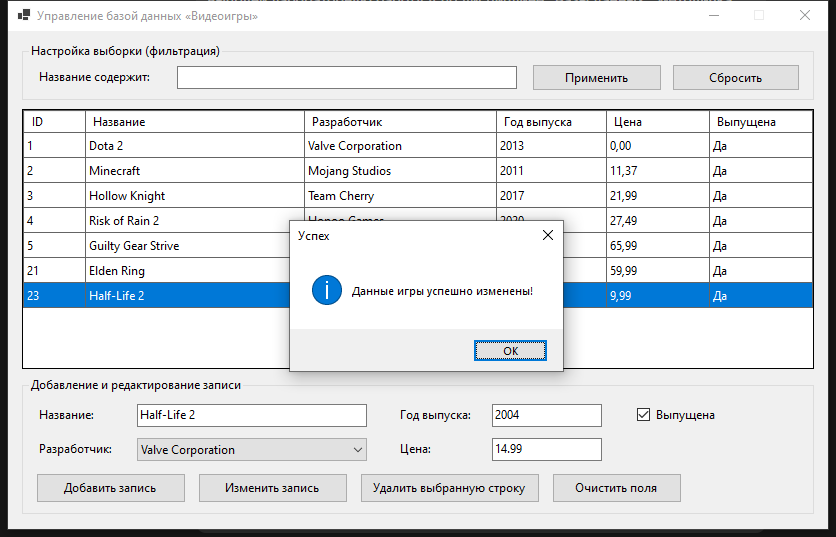
\includegraphics{s5.png}}
		\caption{Изменение данных выбранной записи}
	\end{figure}
	
	Работа регистронезависимого фильтра по строковому значению (ввод подстроки \texttt{hollow} в нижнем регистре находит запись \texttt{Hollow Knight} с помощью SQL-запроса и функции \texttt{UPPER}) представлена на рисунке~7.
	
	\begin{figure}[H]
		\centering
		\adjustbox{max width=0.92\linewidth}{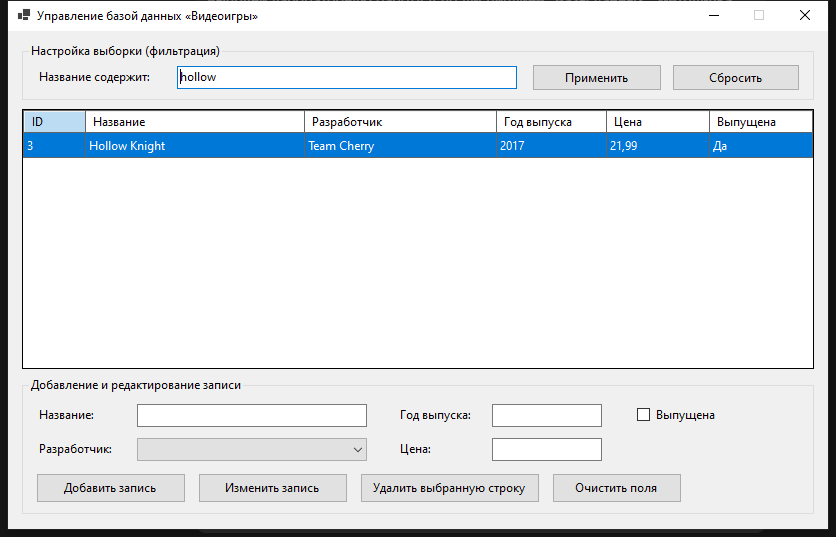
\includegraphics{s6.png}}
		\caption{Регистронезависимая фильтрация записей через запрос к БД}
	\end{figure}
	
	Диалоговое окно подтверждения удаления выбранной строки («Вы действительно уверены, что хотите удалить выбранную запись?» Да/Нет) перед вызовом PL/pgSQL-функции \texttt{lab\_schema.delete\_game} показано на рисунке~8.
	
	\begin{figure}[H]
		\centering
		\adjustbox{max width=0.92\linewidth}{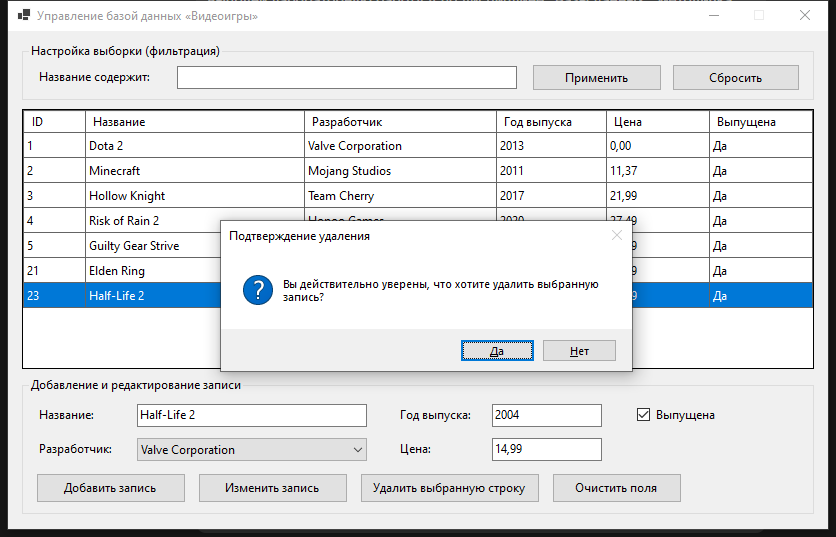
\includegraphics{s7.png}}
		\caption{Подтверждение удаления выбранной записи}
	\end{figure}
	
	\newpage
	
	\section*{Выводы} В ходе выполнения лабораторной работы была изучена библиотека Npgsql для связывания приложения на языке C\# с базой данных под управлением СУБД PostgreSQL. Спроектирована объектно-ориентированная архитектура взаимодействия с базой данных с применением шаблонов проектирования Repository (DAO) и Factory Method, составлена диаграмма разработанных классов. Разработано приложение с русскоязычным графическим интерфейсом Windows Forms для работы с таблицей \texttt{game}, ссылающейся по внешнему ключу на родительскую таблицу \texttt{developer}. Реализованы вывод, добавление, изменение и удаление данных с подтверждением через хранимые функции PL/pgSQL, выбор внешнего ключа по названию из списка родительской таблицы, запрет ввода отрицательных значений, защита от повторной записи уже существующих данных, а также регистронезависимая фильтрация записей через запрос к базе данных с использованием функции \texttt{UPPER}.
	
\end{document}
